% !TEX root = main.tex
\documentclass{article}
\usepackage{float}
\usepackage{graphicx} % Required for inserting images
\usepackage{tabularx}
\usepackage{xltabular}

% Title definition
\title{

    \begin{center}
        
\includegraphics[width=0.5\textwidth]{images/PolimiLogo.png} 
    \end{center}

    \vspace{1cm}
    
    \Huge\bfseries Best Bike Paths\\
    \vspace{0.5cm}
    
    {\Large Design Document (DD)}
}

\author{A. Rubino \and E. Uvinsi \and I. Vinciguerra}
\date{Academic Year 2025/2026}



\begin{document}


\maketitle
\newpage
\tableofcontents
\newpage
\section{INTRODUCTION}
\subsection{Scope}
The core function of the BBP system is to provide a comprehensive, community-driven platform to all types of cyclists. The system acts as an intermediary,
processing heterogeneous data inputs from various sources, including external
providers, and synthesizing this information to generate reliable output for all
users. \\
\noindent The architectural design detailed in this document aims to fulfill the requirements outlined in the RASD document. The BBP system is designed to be scalable, modular, and maintainable, ensuring that it can adapt to future needs and technological advancements. \\
\noindent The design is centered around \textbf{a multi-tier client-server architecture} that separates concerns across different layers, promoting a clear division of responsibilities. This approach enhances the system's ability to handle diverse data sources and user interactions effectively. \\
\noindent The BBP system incorporates various components, each responsible for specific functionalities such as user management, data acquisition, path reconstruction, and path publication. These components interact seamlessly to provide a cohesive user experience while ensuring data integrity and reliability. \\

\subsection{Definitions, Acronyms, Abbreviations}
\subsubsection{Definitions}
\begin{itemize}
    \item \textbf{Global Positioning System}: a satellite-based navigation system owned by the U.S. government that uses a constellation of orbiting satellites, ground control stations, and receivers to provide precise positioning, navigation, and timing information.
    \item \textbf{Accelerometer}: a sensor that measures linear acceleration (changes in velocity over time) along one or more axes.
    \item \textbf{Gyroscope}: a sensor that measures angular velocity. It detects how fast an object is rotating around a specific axis, which is essential for determining a device’s current orientation in space.
    \item \textbf{Meteorological Service Provider}: a formal entity that is responsible for the collection, processing, analysis, forecasting, and dissemination of meteorological and related environmental information and services.
    \item \textbf{Map Service Provider}: a formal entity that provides geospatial infrastructure, data, and rendering capabilities to software applications. It manages the acquisition, storage, and processing of raw Geographic Information Systems (GIS) data such as satellite imagery, vector topology, and traffic signals, allowing client applications to request processed map assets and perform spatial calculations on demand, without maintaining a proprietary geospatial backend.
\end{itemize}

\subsubsection{Acronyms}
\begin{itemize}
    \item \textbf{BBP}: Best Bike Paths
    \item \textbf{RU}: Registered User
    \item \textbf{RASD}: Requirements Analysis and Specification Document
    \item \textbf{DD}: Design Document
    \item \textbf{GPS}: Global Positioning System
    \item \textbf{API}: Application Programming Interface
    \item \textbf{UI}: User Interface
    \item \textbf{JSON}: JavaScript Object Notation
    \item \textbf{REST}: Representational State Transfer
    \item \textbf{HTTP}: HyperText Transfer Protocol
    \item \textbf{HTTPS}: HyperText Transfer Protocol Secure
    \item \textbf{SQL}: Structured Query Language
    \item \textbf{NoSQL}: Not Only SQL
    \item \textbf{GIS}: Geographic Information Systems
    \item \textbf{XML}: eXtensible Markup Language
\end{itemize}

\subsection{Revision History}
\subsection{Document Structure}
\begin{enumerate}
    \item \textbf{Introduction}: This section aims to give a brief description of the project. In particular it offers an overview of the purpose of the document and a very general description of the adopted solution.
    \item \textbf{Architectural Design}: This part of the document describes at different levels of granularity how the architecture is designed.
    \item \textbf{User Interface Design}: This section shows the wire frame that constitutes the platform UI.
    \item \textbf{Requirements Traceability}: This section contains the traceability matrix that maps the requirements to the components that implement them.
    \item \textbf{Implementation, Integration and Test Plan}: This section provides a description of the implementation integration and testing details, useful for the developers and producer of the platform.
    \item \textbf{Effort Spent}: It contains a table that shows the effort spent to write this document.
    \item \textbf{References}: It contains the references to any documents and software used to write this document.
\end{enumerate}
\section{ARCHITECTURAL DESIGN}

\subsection{Overview: High level components and their interaction}
\noindent\makebox[\textwidth][c]{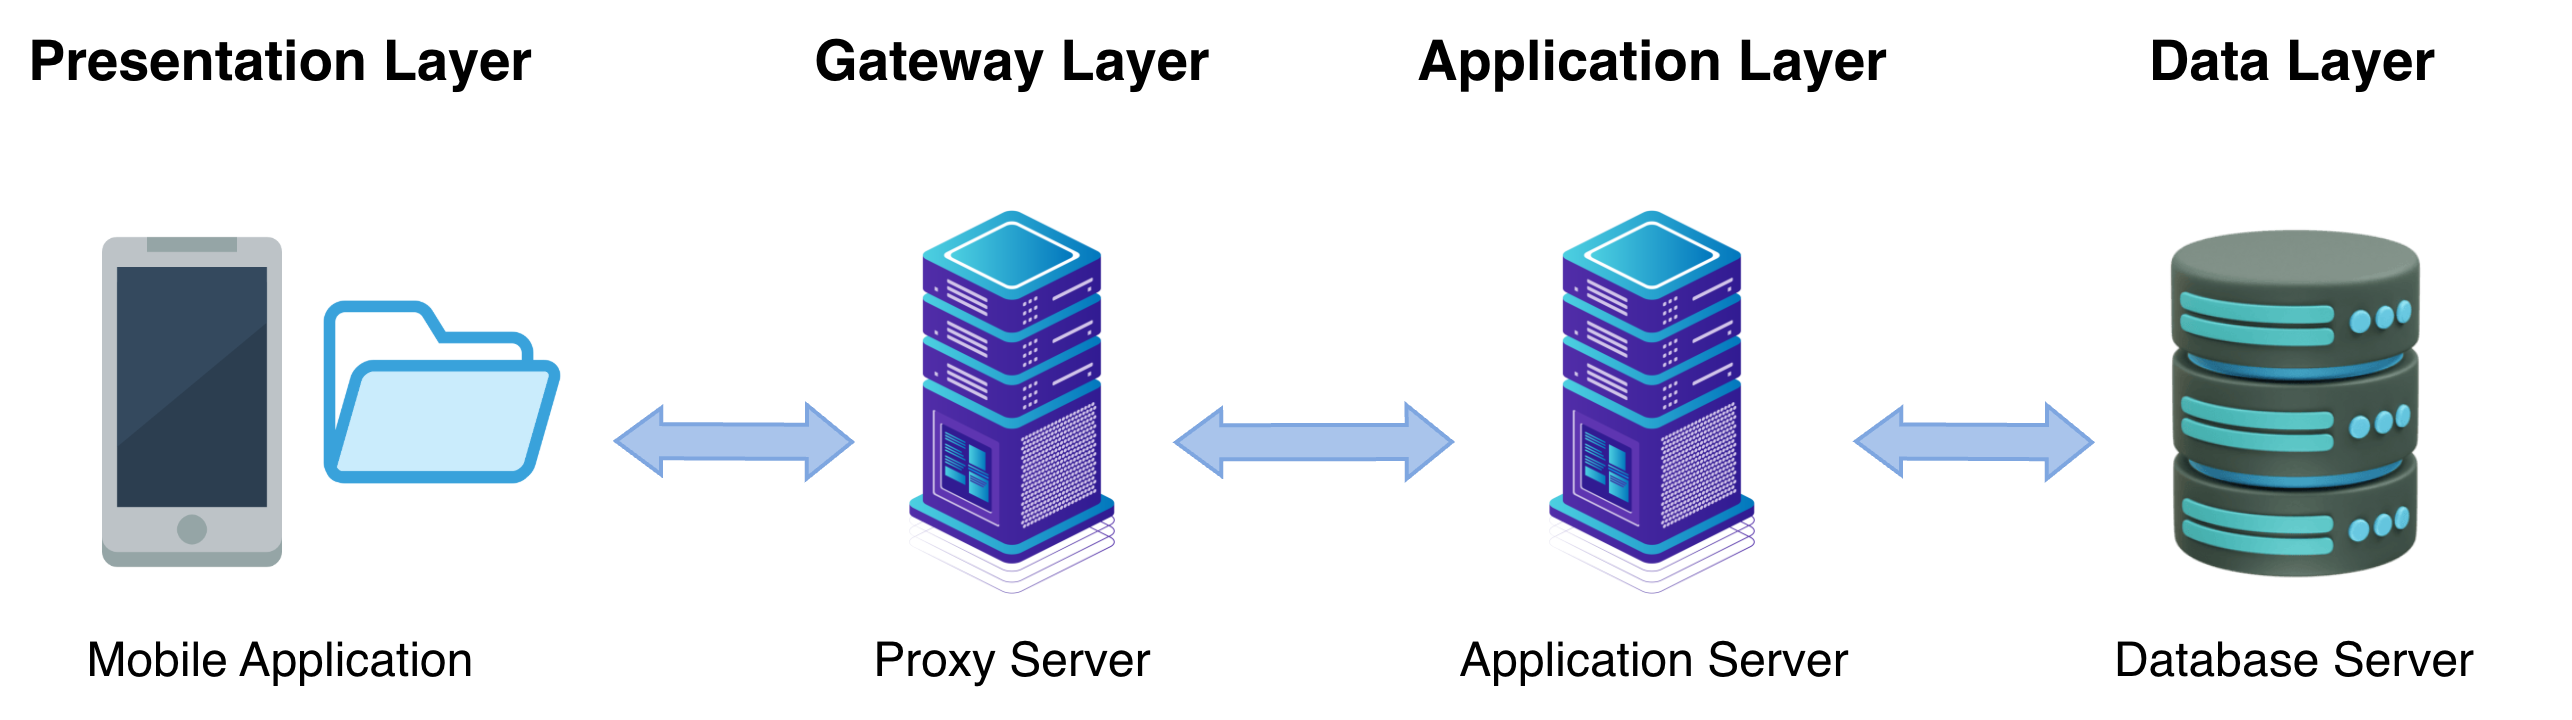
\includegraphics[width=1.1\textwidth]{images/InformalDiagram.png}}
\subsection{Component view}
%Introduzione generale ai componenti. Architettura client-server 3 livelli (min) distribuita
%Server distribuiti geograficamente. GUI e salvataggi percorsi privati esclusivamente in locale (dunque parte del db in locale)
%Ricerca dei percorsi tramite server

\begin{itemize}
    \item \textbf{User Management Service}
    \item \textbf{Automated Path Data Collection Service}
    \item \textbf{Path Data Transformation Service} %trasforma i dati raw collezionati dai sensori in un formato human readable
    \item \textbf{Meteorological Data Retrieval Service}
    \item \textbf{Path Research Service} %unico riservato anche a utenti non registrati
    \item \textbf{Path Publication Service}
    \item \textbf{Manual Path Insertion Service}
    \item \textbf{Inventory Handling Service}
\end{itemize}

\newpage
\subsection{Deployment view}
This chapter describes the deployment view of the BPP system. it outlines the execution
environment of the system and details the gegraphical distribution of the hardware components that host the
software making up the application. 
\noindent\makebox[\textwidth][c]{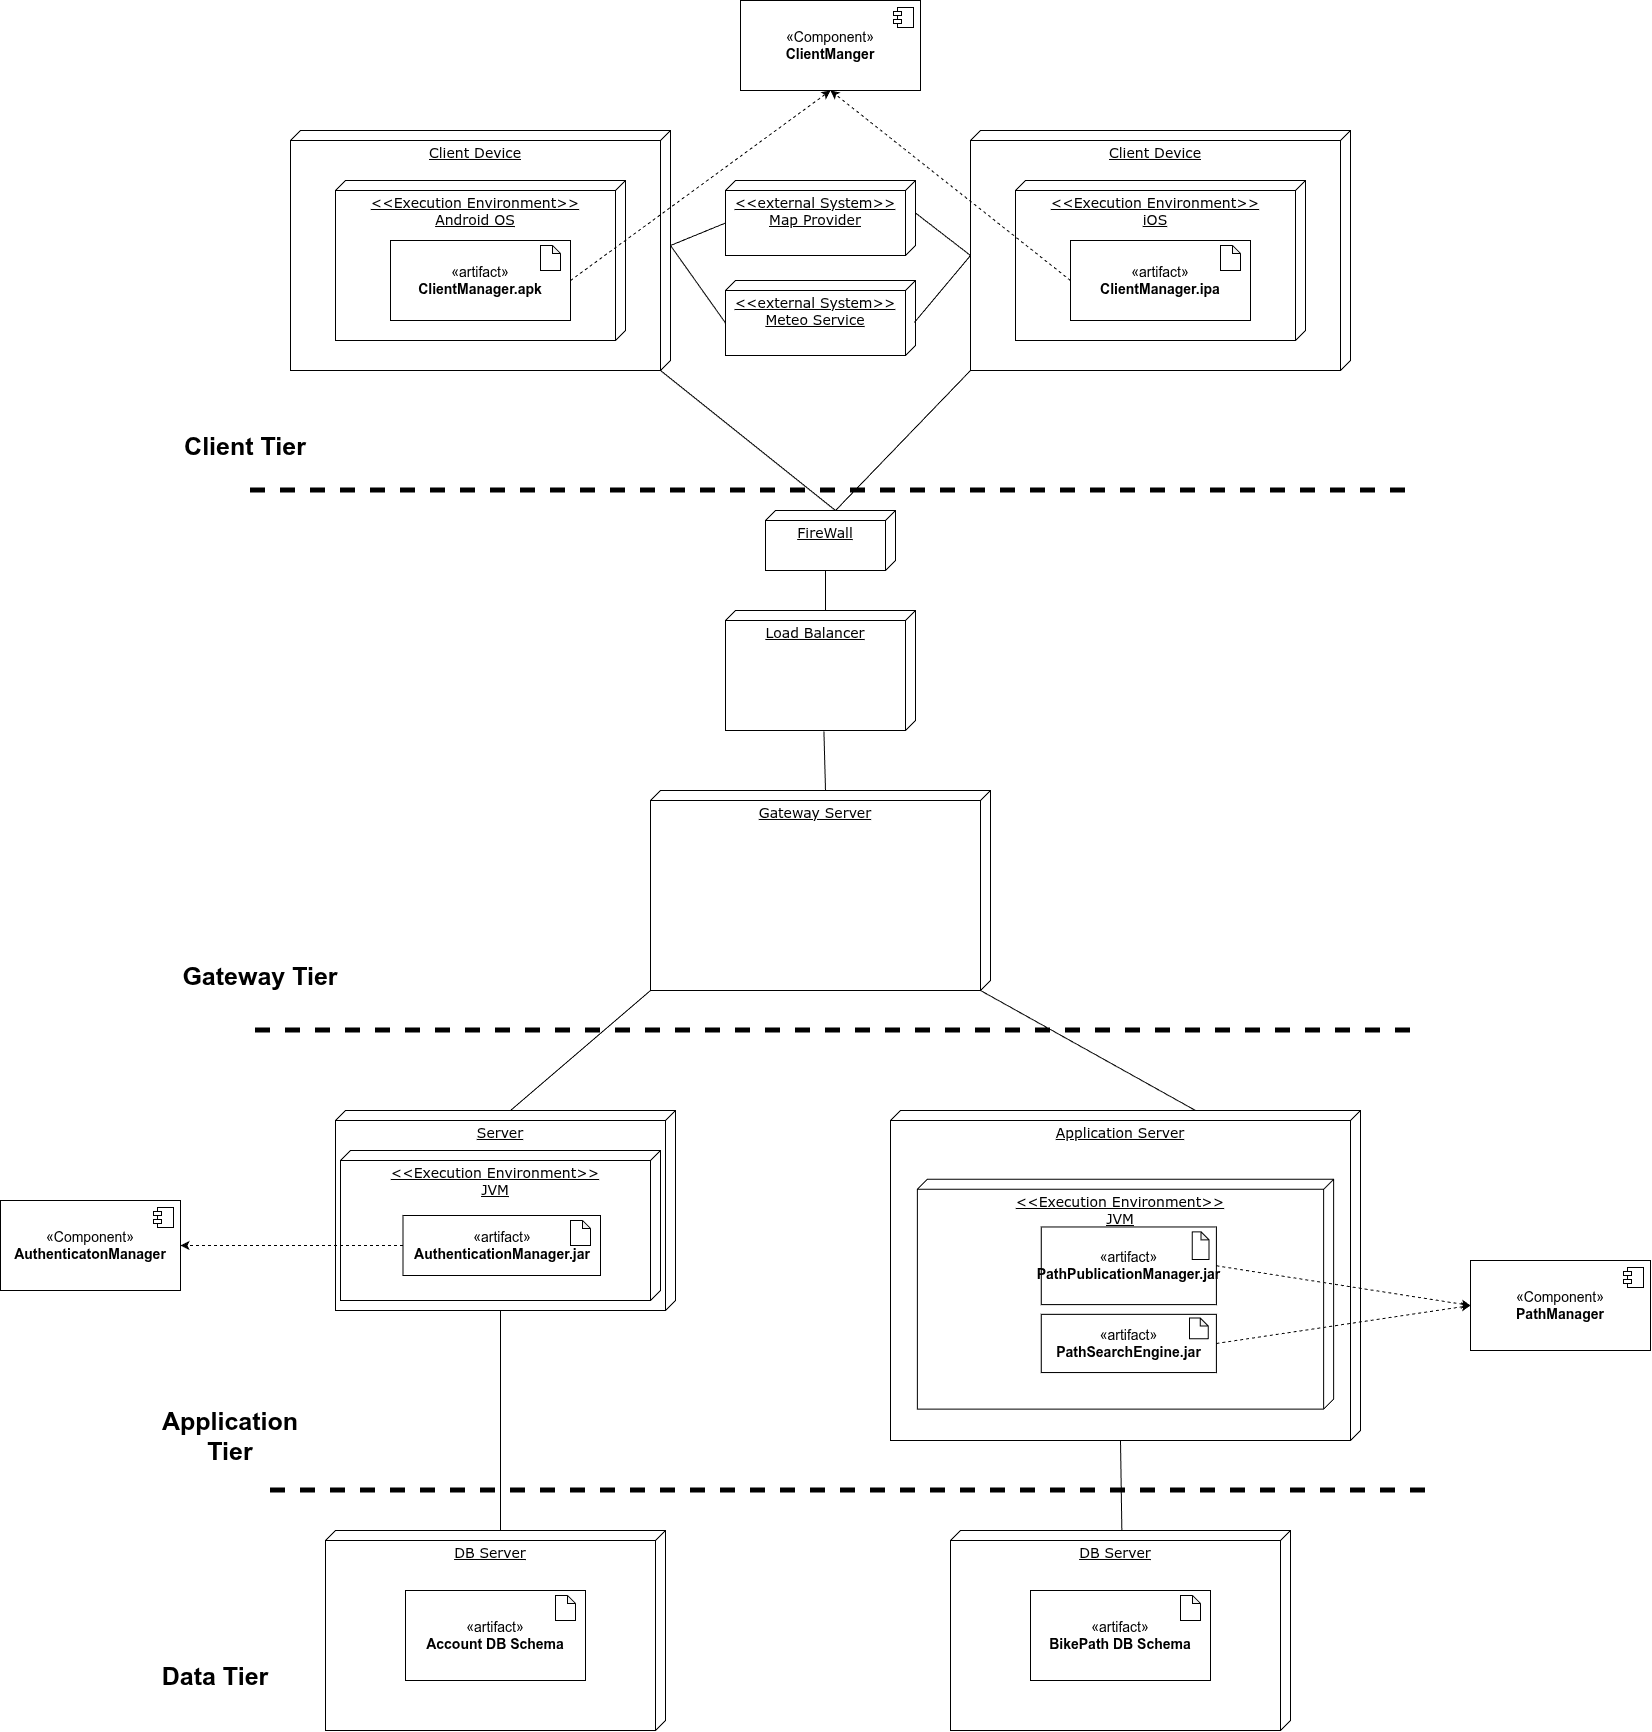
\includegraphics[width=1.1\textwidth]{images/Deployment_Diagram.drawio.png}}

\newpage \noindent The deployment architecture follows a Four-Tier approach. The first tier is a Thick Client able to provide parts of the functionalities (gathering of
information and offline storage) also when it is not connected to the Server. \newline\newline
The second tier consists of the Gateway and the Load balancer. The Gateway exposes the public endpoint and route the requests toward the 
correct type of service (Account Server or Application Server). This layer works also as shield against external treats. The communication between first and second tier takes
place via HTTPS protocol.\newline\newline
The third tier consist of two types of servers: The ones to manage all the things regarding the personal account of a user and the ones that regard the "shared" part of the application, i.e. the publication of bike paths.
This separation between the two aspect allow to easily achieve independent scalability of the two type of service, and allow the system to avoid the congestion of both service if only one is managing a big quantity of requests. In other words this kind of
separation introduces a high level of decoupling.
The fourth and last tier is dedicated to the Data, the databases do not communicate directly with internet but only with the Servers responsible to manage the information.\newline
The communication between these tiers takes place via TCP/IP protocol.\newline\newline

We proceed to provide further details about the elements in the graph. \newline\newline



\begin{itemize}
    \item \textbf{Database Server for Published Paths} \\
    This database stores all the published paths by registered users.
    The system shall be highly available and shall be able to provide eventual consistency across all the
    replicas, so all the set of available paths will be visible to all the users around the world.
    \item \textbf{Database Server for Registered Users} \\
    This Database stores all the personal information of registered users such as name, e-mail and the hashed password.
    \item \textbf{Application Server}\\
    This Server is responsible to process all the requests regarding the publication and the search of bike path from the final user.
    This component manipulates data, and then it has direct access to the related Database.
    \item \textbf{Account Server}\\
    This Server is responsible to manage all the request that regard the accounts of the end user and the related information.
    This component manipulates personal data of the users, and then it has access to the related Database.
    \item \textbf{Load Balancer} \\
    It distributes incoming requests across multiple Gateway to optimize system performances and avoid to overloading one server.
    \item \textbf{Firewall}\\ %Ops... non ci sono nel deployment diagram <-- Sistema
    Monitors incoming network traffic, blocking potentially harmful packets before they reach the system. Positioned before the load balancers it creates
    a safe perimeter around the network.
    \item \textbf{Mobile Device} \\
    This represents the device used by the end user. It requires the app installed in order to access the BPP application. 
\end{itemize}
\subsection{Runtime view}
\subsection{Component interfaces}
\subsection{Selected architectural styles and patterns}
\subsection{Other design decisions}
\section{USER INTERFACE DESIGN}

This chapter illustrates the user interface mockups. Specifically, it revisits 
the mockups originally presented in the RASD, supplementing them with additional 
screens to provide a more design-oriented perspective. \\

\noindent Displayed below is the initial screen encountered upon launching the mobile application. As can be observed, this 
interface offers the option to log in (located at the top) or to proceed in Guest Mode 
(shown at the bottom). As previously stated, Guest Mode is restricted; consequently, 
users operating in this mode are limited solely to searching for paths within the BBP 
system database.

\begin{figure}[H]
    \centering
    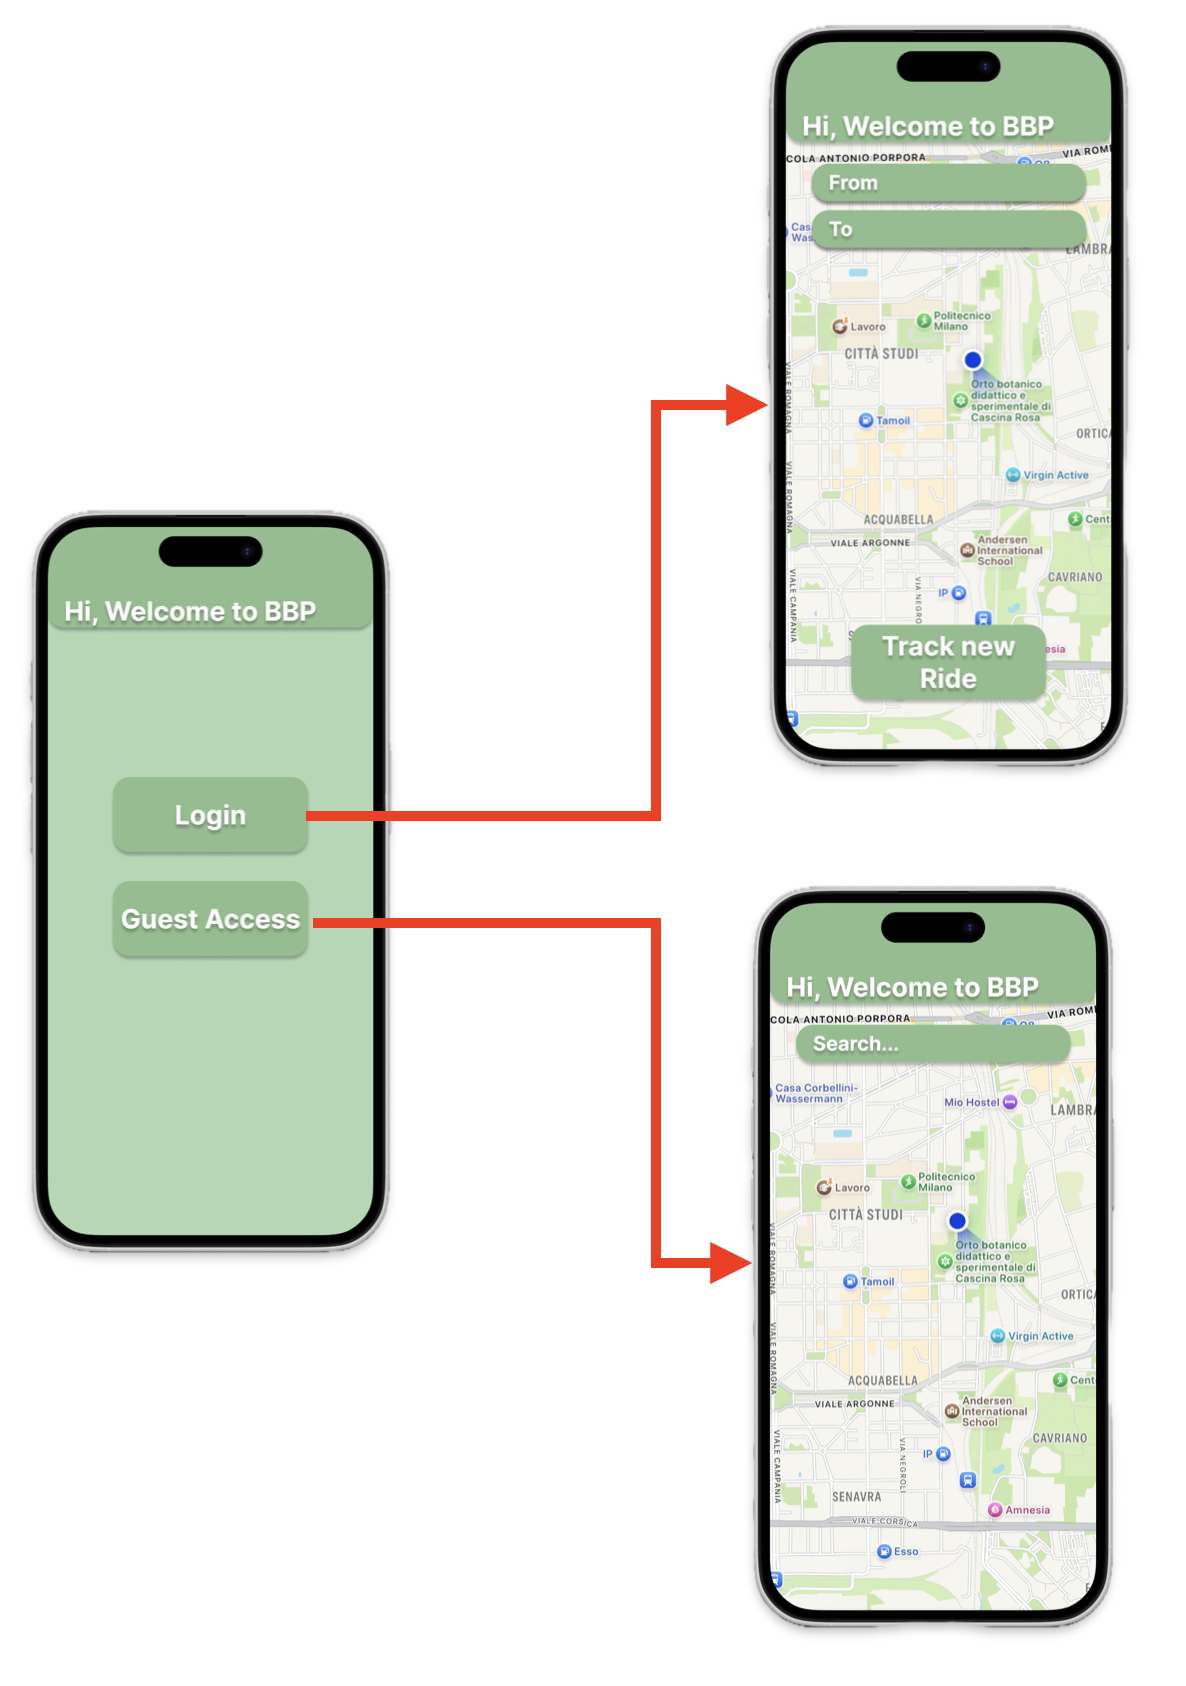
\includegraphics[width=0.5\textwidth]{images/prototype1.png}
    \caption{Homepage screen mockup}
    \label{fig:startup_mockup}
\end{figure}    

\noindent The following screens present the general workflow, illustrating the two tracking 
alternatives available for recording a new ride: automatic and manual. Specifically, 
upon clicking 'Track New Ride', the user is given the option to select the data acquisition 
mode. \\

\noindent If manual mode is selected (illustrated at the top), the user is presented with 
a form to sequentially enter each street (or street segment) and its corresponding status. 
Upon completing this process and confirming, the user is directed to a preview screen.\\

\noindent A similar screen is also displayed to users who, after selecting automated mode, 
decide to terminate the session (or when the system detects inactivity and automatically 
interrupts data acquisition). \\

\noindent In either scenarios, once on the preview screen, the user can 
further refine the manually entered or automatically detected data. In the second case, the refinement is mandatory. Finally, the user can choose 
to press 'Exit' to discard the collected data or 'Save' to store the acquired data locally. 
Should the latter option be selected, the user must be offered the choice to either publish 
the path or keep it private, making it viewable solely by them within their personal records log.\\

\begin{figure}[H]
    \centering
    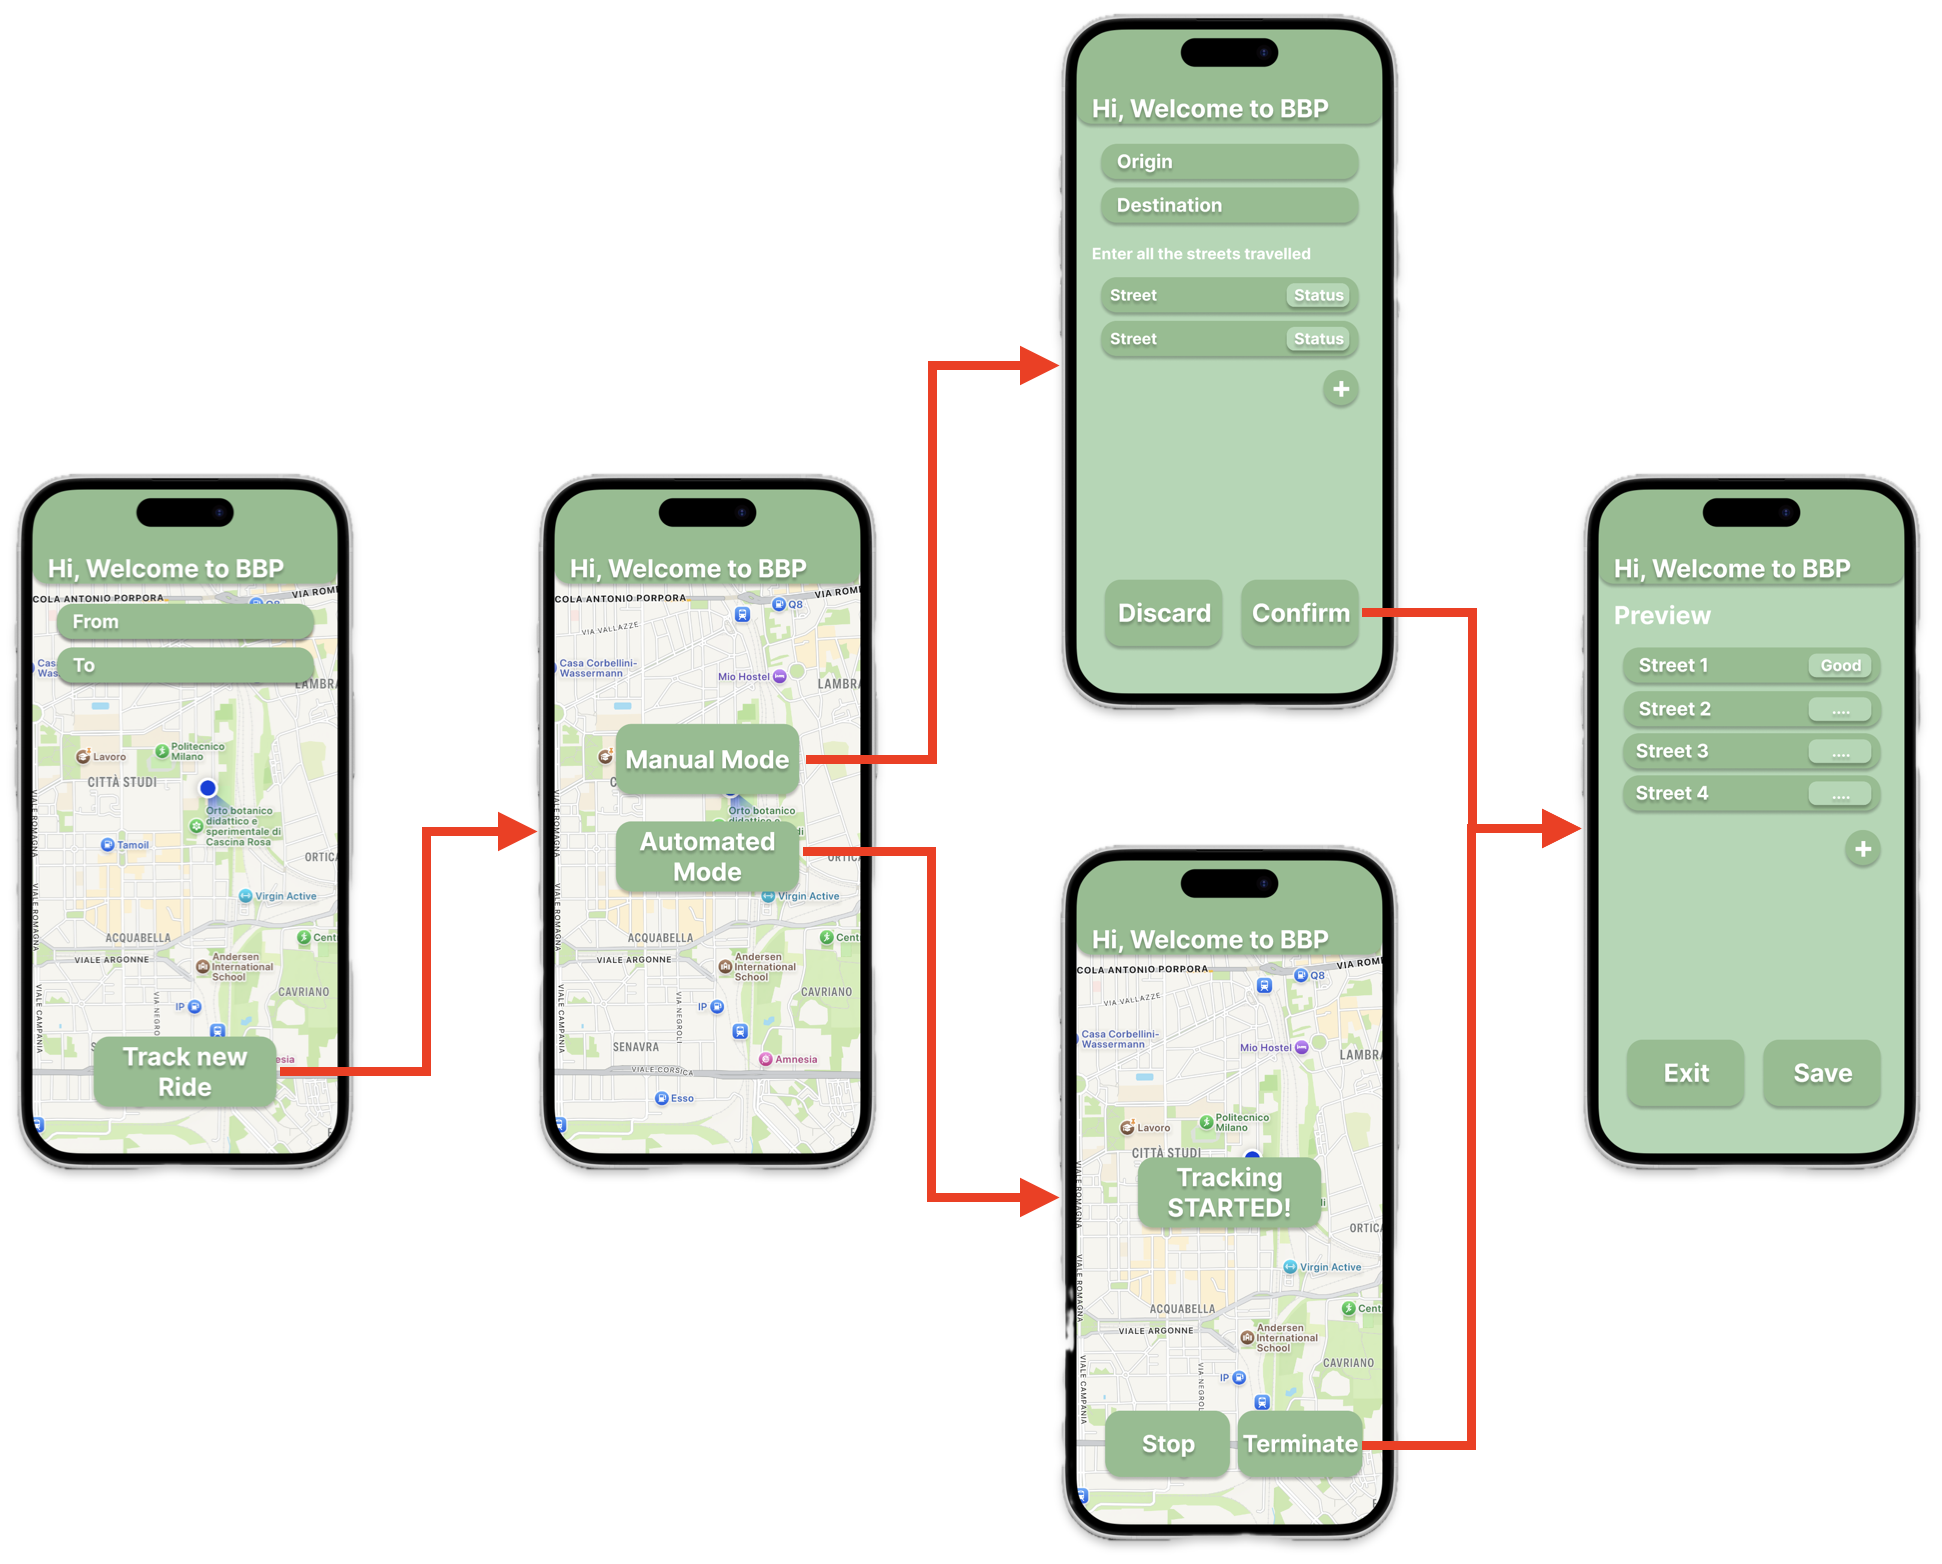
\includegraphics[width=1\textwidth]{images/prototype2.png}
    \caption{Tracking mode selection screen mockup}
    \label{fig:loggedin_mode_mockup}
\end{figure}

\noindent We now examine the automated path tracking workflow in greater detail. As can be observed, the first 
four screens are identical to those presented in the previous figure; indeed, the focus here is 
specifically on the final phase of the tracking process. In this stage, the user views the path 
preview and, after optionally refining the data, chooses to save the path, at which point they are 
presented with the option to immediately publish the record. \\

\begin{figure}[H]
    \centering
    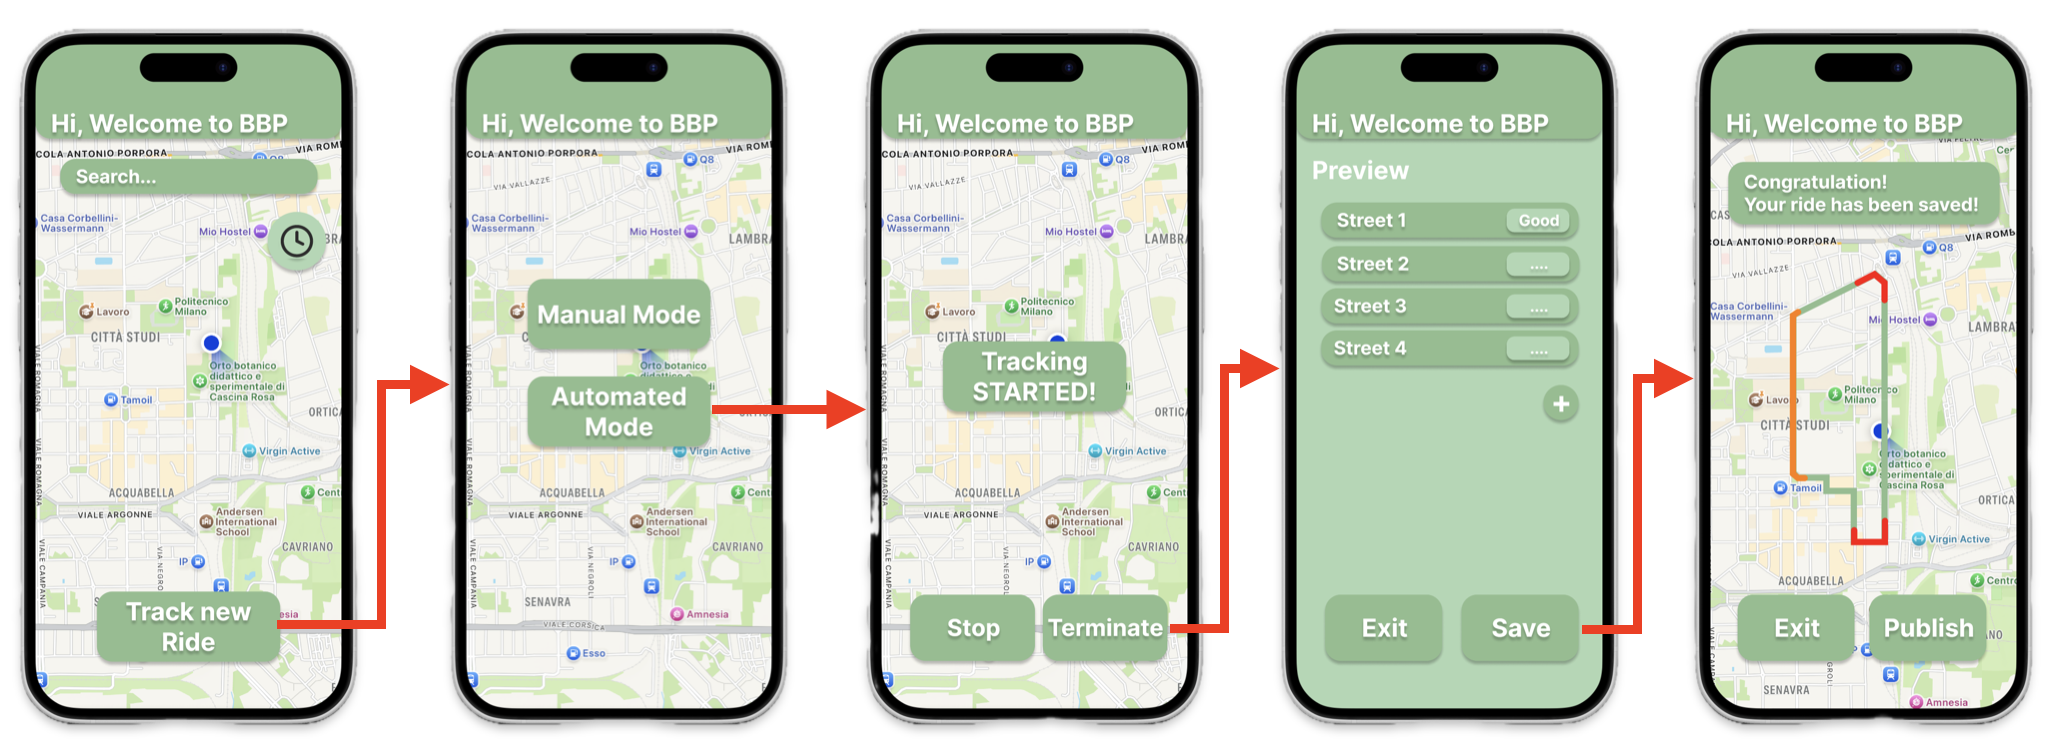
\includegraphics[width=1\textwidth]{images/prototypeAUTOMATED.png}
    \caption{Automated tracking screen mockup}
    \label{fig:Automated_tracking_mockup}
\end{figure}    

\noindent Proceeding further, we encounter the workflow for viewing a specific record within the sessions inventory. Specifically, the Home Screen features a button that grants access to the complete list of 
records. From this list, users can view the details of individual record, as depicted in the final 
screen on the right. This screen displays a hypothetical map that graphically highlights the path 
and indicates the status of its constituent streets.\\

\noindent This interface also allows users to review their performance metrics, which are obtained from the acquired data. Furthermore, within this view, the user must be provided with the option to modify the 
path's publication status (i.e., publishing a private path or reverting a public path to private
if the user no longer wishes to share it) and, if necessary, to delete the record entirely. \\

\noindent It should be noted that these mockups are purely illustrative and may not explicitly depict every detailed of the described features, especially under the design point of view.\\

\begin{figure}[H]
    \centering
    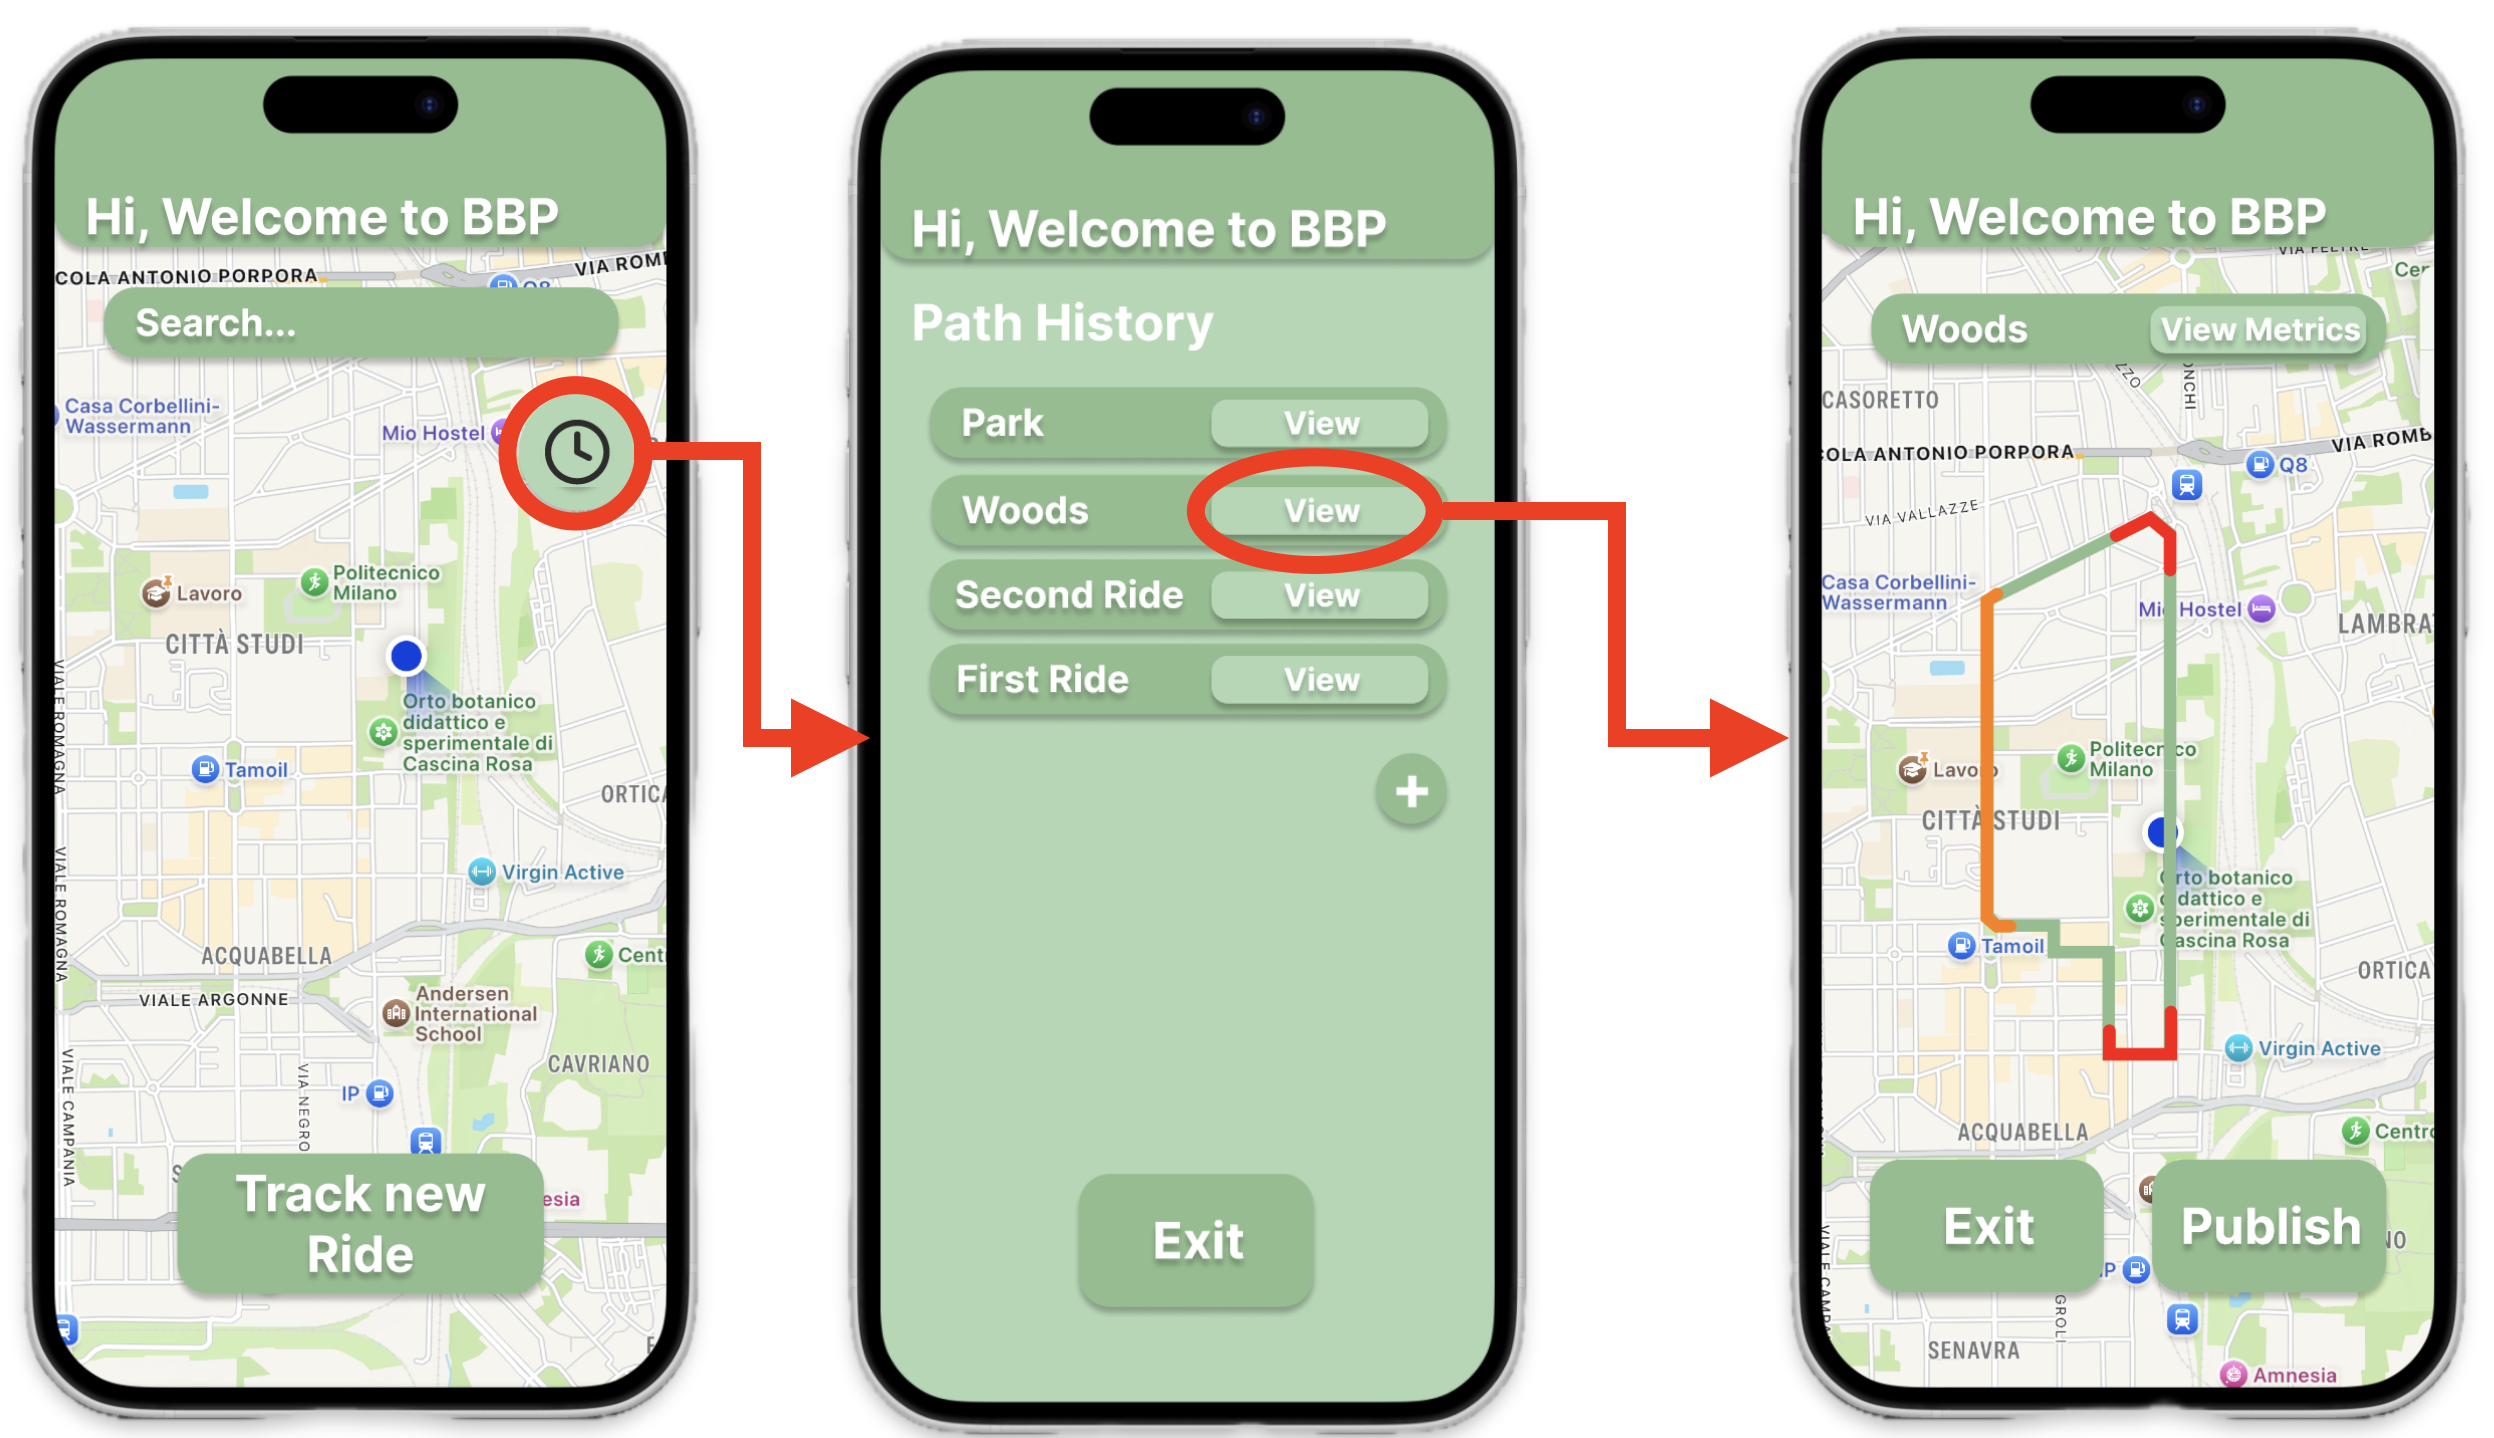
\includegraphics[width=1\textwidth]{images/prototypeVIEWRECORDS.png}
    \caption{View recorded ride screen mockup}
    \label{fig:view_recorded_ride_mockup}
\end{figure}

\noindent Finally, the last figure illustrates the path search workflow. As can be observed, the diagram 
deliberately depicts the scenario where the user is in Guest Mode. Consequently, starting from 
the main screen, the user clicks on 'Search,' enters the origin and destination, and is presented 
with a list of paths sharing similar origins and destinations, ranked by score.\\

\noindent From this list, the user has the option to press 'View' to examine the path's details and its 
associated score. It is important to note that the workflow is analogous for logged-in users. 
The primary distinction is that logged-in users, upon accessing the path detail screen, may be 
offered the option to immediately launch automatic tracking while being redirected to a third-party map application to get geographical directions; this is considered a useful but 
optional shortcut, and its inclusion is therefore left to the discretion of the implementer. \\

\begin{figure}[H]
    \centering
    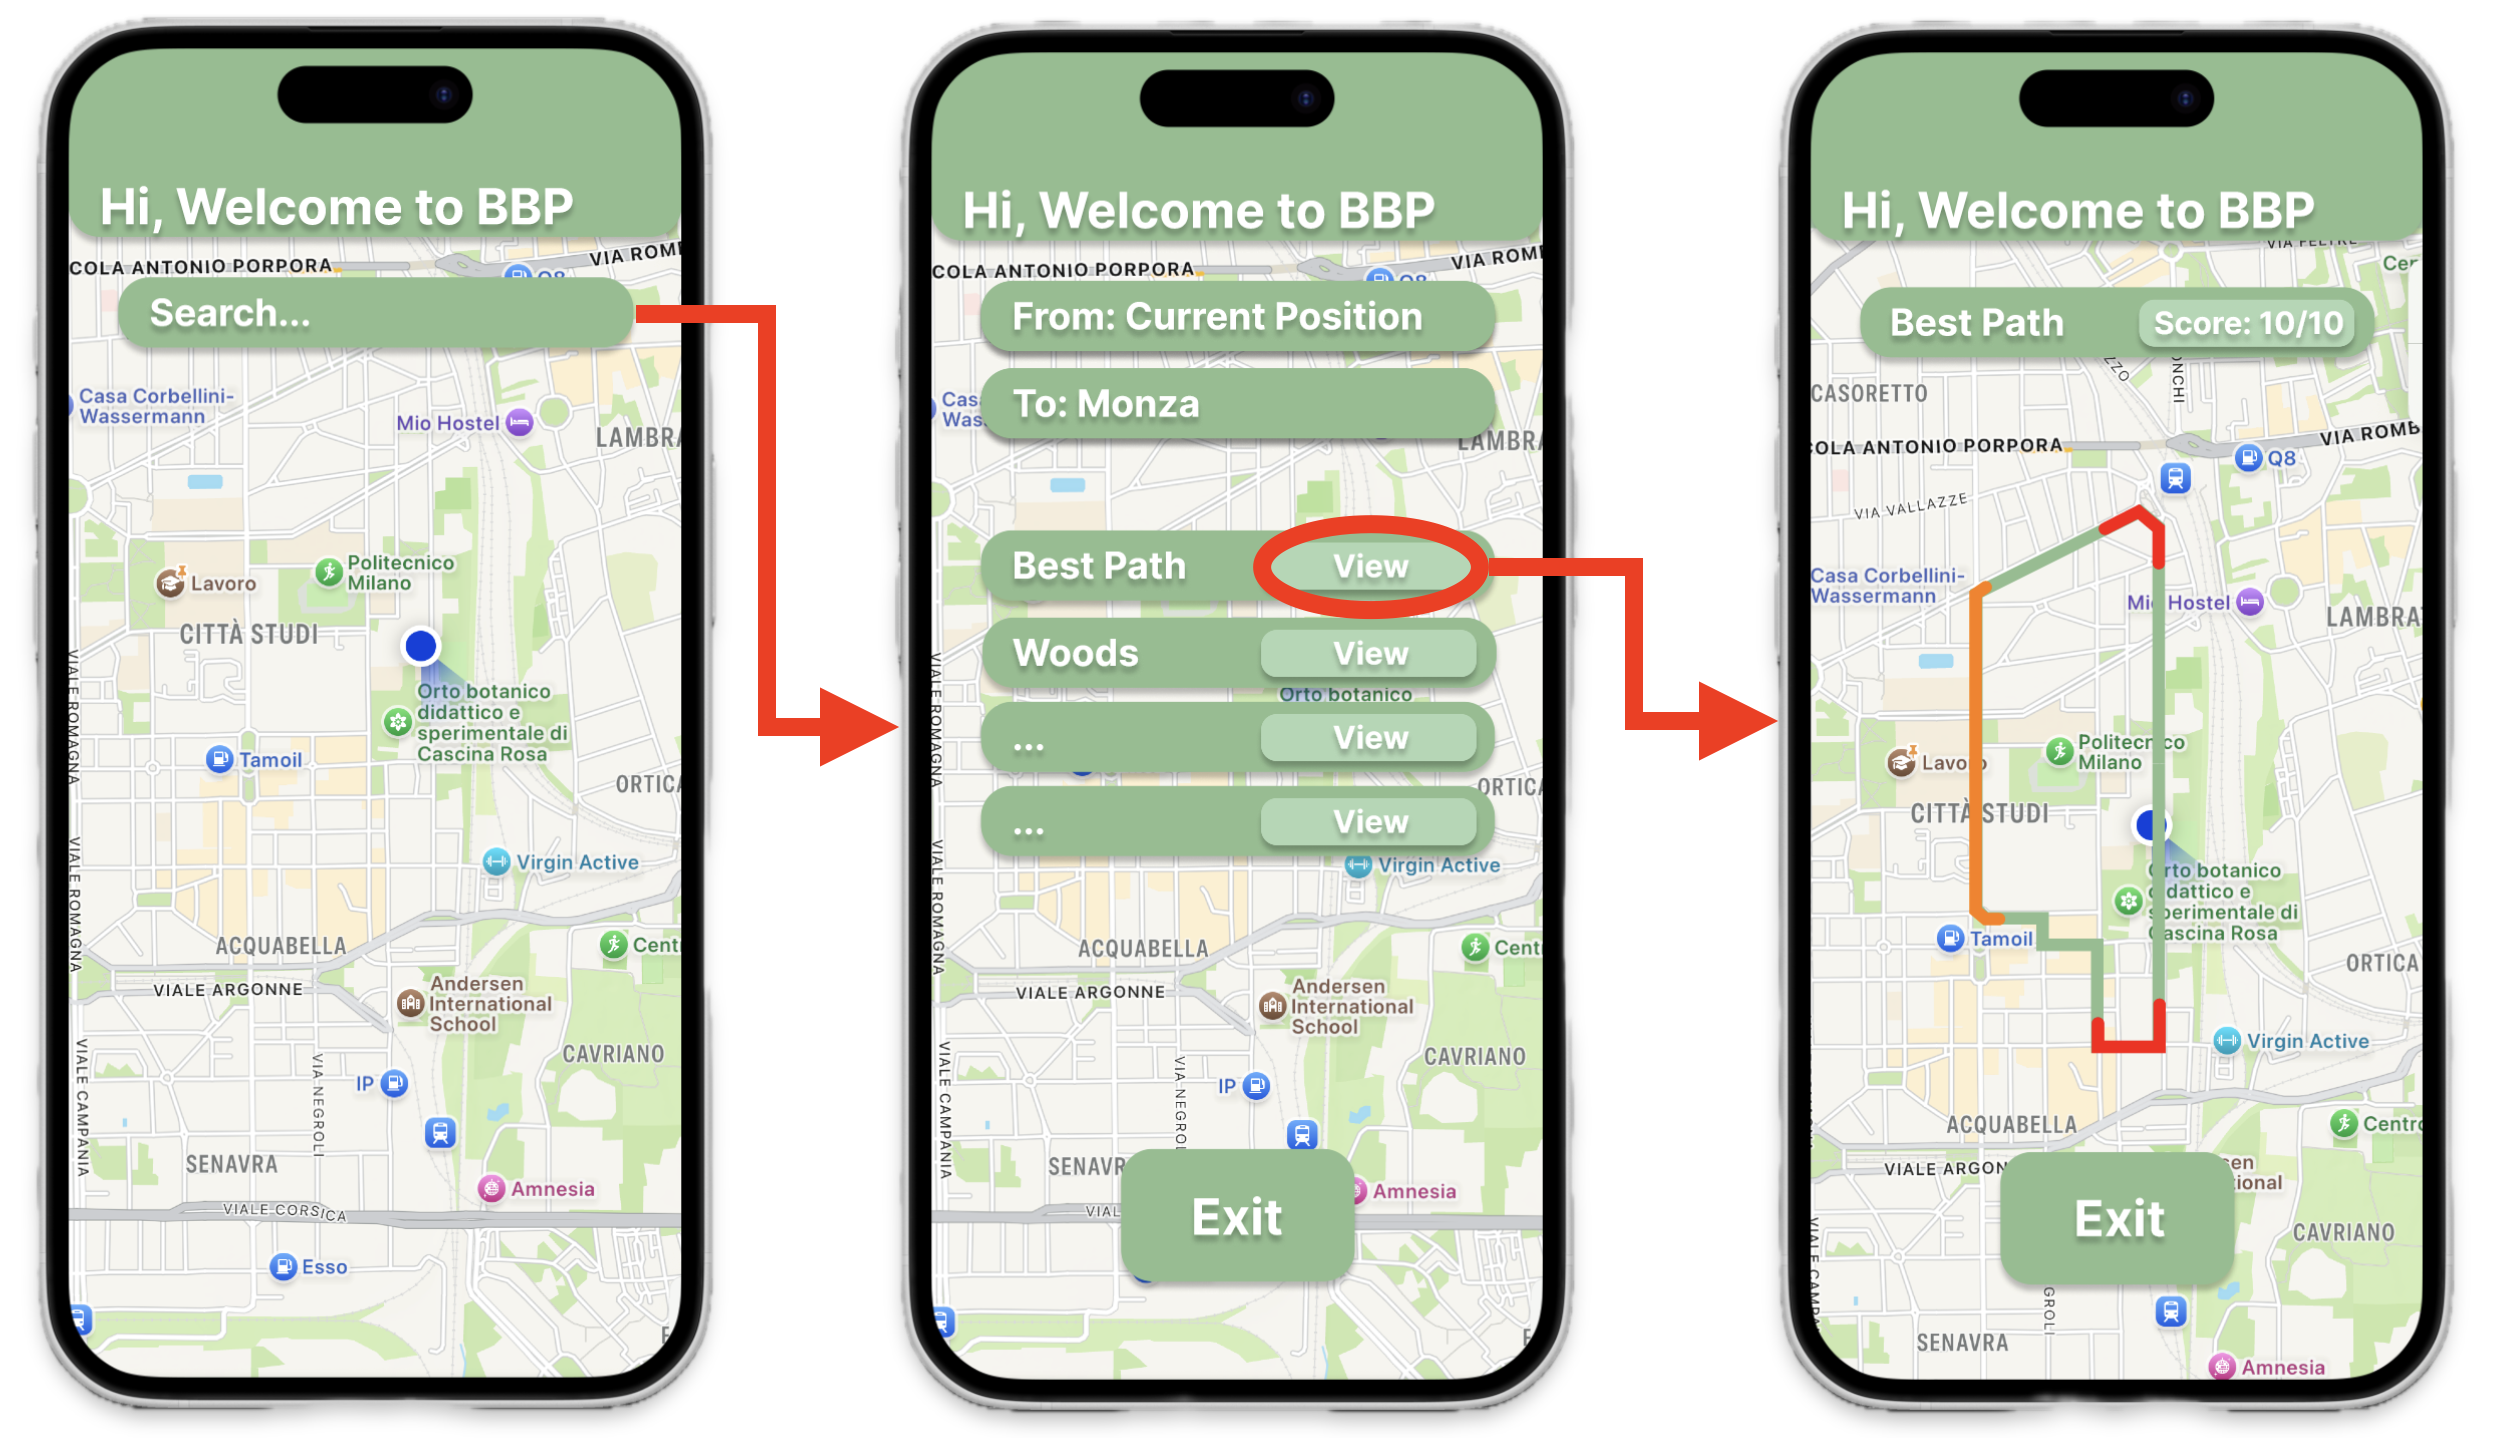
\includegraphics[width=1\textwidth]{images/prototypeSEARCHFORAPATH.png}
    \caption{Search for a bike path screen mockup}
    \label{fig:search_for_a_bike_path_mockup}
\end{figure}

\noindent It is repeated again for the sake of clarity that the mockups do not represent a strict set of guidelines to be followed in absolute terms during the implementation phase, 
but rather a starting point intended to clarify design choices and eliminate residual ambiguities.
\section{REQUIREMENTS TRACEABILITY}

\begin{table}[H]
\centering
\renewcommand{\arraystretch}{1.5} 
\begin{tabular}{|p{0.50\textwidth}|p{0.45\textwidth}|}
\hline
\textbf{Requirements} & \textbf{Design Elements} \\
\hline

\textbf{Access and Users Management} \newline
R1: Create account \newline
R2: Distinguish/Manage authorization & 
User Management Service \newline
Account Server \newline
Database Server for Registered Users \\
\hline

\textbf{Data Acquisition and Validation} \newline
R3: Initiate trip tracking \newline
R4: Pause trip tracking \newline
R5: Terminate trip tracking \newline
R6: Collect data (GPS, gyroscope, accelerometer) \newline
R9: Monitor speed to detect activity & 
Automated Path Data Collection Service \newline
Mobile Device \\
\hline

\textbf{Path reconstruction and metrics} \newline
R7: Reconstruct path from GPS data \newline
R8: Signal presence of obstacles \newline
R16: Compute performance metrics & 
Path Data Transformation Service \\
\hline

\textbf{External Data} \newline
R10: Retrieve meteorological information & 
Meteorological Data Retrieval Service \\
\hline

\textbf{Manual Input} \newline
R13: Retrieve and validate manual street data & 
Manual Path Insertion Service \newline
Mobile Device \\
\hline

\textbf{Local Data Management} \newline
R12: Correct data before publication \newline
R15: Keep private log of tracked sessions & 
Inventory Handling Service \newline
Mobile Device \\
\hline

\textbf{Publication, Scoring \& Merging} \newline
R11: Manual confirmation before publish \newline
R14: Publish manually submitted data \newline
R17: Calculate path's score \newline
R18: Score computation logic \newline
R23: Merge information for same streets \newline
R24: Information merge logic & 
Path Publication Service \newline
Application Server \newline
Database Server for Published Paths \\
\hline

\textbf{Browsing and Search} \newline
R19: Display paths in order of score \newline
R20: Display paths within radius \newline
R21: Edit accuracy radius \newline
R22: View published path data & 
Path Research Service \newline
Application Server \newline
Database Server for Published Paths \\
\hline

\end{tabular}
\label{tab:req_traceability}
\end{table}
\section{IMPLEMENTATION, INTEGRATION AND TESTING}

\subsection{Overview}
\subsection{Implementation Plan}
\subsection{Features identification}
\subsection{Component Integration and Testing}
\subsection{System Testing}
\subsection{Additional Specifications on Testing}


\section{EFFORT SPENT}
The following table shows the approximate amount of hours that each group member spent on each chapter of this document. Please note that is calculation is only approximate, as each section still required active collaboration from all group members.
\begin{table}[h]
    \centering
    % \caption{Effort Spent (Hours)}
    \label{tab:effort}
    \begin{tabular}{|l|c|c|c|c|c|}
        \hline
        \textbf{Group Member} & \textbf{Chapter 1} & \textbf{Chapter 2} & \textbf{Chapter 3} & \textbf{Chapter 4} & \textbf{Chapter 5}\\
        \hline
        A. Rubino & 1 & 15 & 1 & 1 & 8 \\
        \hline
        E. Uvinsi & 1 & 20 & 5 & 3 & 1\\
        \hline
        I. Vinciguerra & 2 & 10 & 1 & 1 & 1\\
        \hline
        \textbf{TOT} & \textbf{4} & \textbf{45} & \textbf{7} & \textbf{5} & \textbf{10} \\
        \hline
    \end{tabular}
\end{table}

\section{REFERENCES}
\begin{enumerate}
    \item \textbf{Project documents}:
        \begin{itemize}
            \item Specification document for the 2025/26 RASD project for the Software Engineering II course.
            \item Slides on the WeBeep page of the Software Engineering II course.
        \end{itemize}
    \item \textbf{Standards and regulations}:
        \begin{itemize}
            \item GDPR (General Data Protection Regulation).
        \end{itemize}
    \item \textbf{External service provider documentation/APIs}:
        \begin{itemize}
            \item Documentation or specifications for the MSP.
            \item Any specific API documentation or licensing terms mentioned for third-party software, libraries, or commercial mapping APIs.
        \end{itemize}
    \item \textbf{Technical specification documentation} for the following tools/protocols/formats:
        \begin{itemize}
            \item Standard geospatial data formats (including GPX - GPS Exchange Format)
            \item REST architectural style for web APIs
            \item HTTP/1.1 and HTTPS
            \item TCP/IP
            \item TLS 1.3
            \item JSON
        \end{itemize}
\end{enumerate}

\end{document}